\documentclass[1p]{elsarticle_modified}
%\bibliographystyle{elsarticle-num}

%\usepackage[colorlinks]{hyperref}
%\usepackage{abbrmath_seonhwa} %\Abb, \Ascr, \Acal ,\Abf, \Afrak
\usepackage{amsfonts}
\usepackage{amssymb}
\usepackage{amsmath}
\usepackage{amsthm}
\usepackage{scalefnt}
\usepackage{amsbsy}
\usepackage{kotex}
\usepackage{caption}
\usepackage{subfig}
\usepackage{color}
\usepackage{graphicx}
\usepackage{xcolor} %% white, black, red, green, blue, cyan, magenta, yellow
\usepackage{float}
\usepackage{setspace}
\usepackage{hyperref}

\usepackage{tikz}
\usetikzlibrary{arrows}

\usepackage{multirow}
\usepackage{array} % fixed length table
\usepackage{hhline}

%%%%%%%%%%%%%%%%%%%%%
\makeatletter
\renewcommand*\env@matrix[1][\arraystretch]{%
	\edef\arraystretch{#1}%
	\hskip -\arraycolsep
	\let\@ifnextchar\new@ifnextchar
	\array{*\c@MaxMatrixCols c}}
\makeatother %https://tex.stackexchange.com/questions/14071/how-can-i-increase-the-line-spacing-in-a-matrix
%%%%%%%%%%%%%%%

\usepackage[normalem]{ulem}

\newcommand{\msout}[1]{\ifmmode\text{\sout{\ensuremath{#1}}}\else\sout{#1}\fi}
%SOURCE: \msout is \stkout macro in https://tex.stackexchange.com/questions/20609/strikeout-in-math-mode

\newcommand{\cancel}[1]{
	\ifmmode
	{\color{red}\msout{#1}}
	\else
	{\color{red}\sout{#1}}
	\fi
}

\newcommand{\add}[1]{
	{\color{blue}\uwave{#1}}
}

\newcommand{\replace}[2]{
	\ifmmode
	{\color{red}\msout{#1}}{\color{blue}\uwave{#2}}
	\else
	{\color{red}\sout{#1}}{\color{blue}\uwave{#2}}
	\fi
}

\newcommand{\Sol}{\mathcal{S}} %segment
\newcommand{\D}{D} %diagram
\newcommand{\A}{\mathcal{A}} %arc


%%%%%%%%%%%%%%%%%%%%%%%%%%%%%5 test

\def\sl{\operatorname{\textup{SL}}(2,\Cbb)}
\def\psl{\operatorname{\textup{PSL}}(2,\Cbb)}
\def\quan{\mkern 1mu \triangleright \mkern 1mu}

\theoremstyle{definition}
\newtheorem{thm}{Theorem}[section]
\newtheorem{prop}[thm]{Proposition}
\newtheorem{lem}[thm]{Lemma}
\newtheorem{ques}[thm]{Question}
\newtheorem{cor}[thm]{Corollary}
\newtheorem{defn}[thm]{Definition}
\newtheorem{exam}[thm]{Example}
\newtheorem{rmk}[thm]{Remark}
\newtheorem{alg}[thm]{Algorithm}

\newcommand{\I}{\sqrt{-1}}
\begin{document}

%\begin{frontmatter}
%
%\title{Boundary parabolic representations of knots up to 8 crossings}
%
%%% Group authors per affiliation:
%\author{Yunhi Cho} 
%\address{Department of Mathematics, University of Seoul, Seoul, Korea}
%\ead{yhcho@uos.ac.kr}
%
%
%\author{Seonhwa Kim} %\fnref{s_kim}}
%\address{Center for Geometry and Physics, Institute for Basic Science, Pohang, 37673, Korea}
%\ead{ryeona17@ibs.re.kr}
%
%\author{Hyuk Kim}
%\address{Department of Mathematical Sciences, Seoul National University, Seoul 08826, Korea}
%\ead{hyukkim@snu.ac.kr}
%
%\author{Seokbeom Yoon}
%\address{Department of Mathematical Sciences, Seoul National University, Seoul, 08826,  Korea}
%\ead{sbyoon15@snu.ac.kr}
%
%\begin{abstract}
%We find all boundary parabolic representation of knots up to 8 crossings.
%
%\end{abstract}
%\begin{keyword}
%    \MSC[2010] 57M25 
%\end{keyword}
%
%\end{frontmatter}

%\linenumbers
%\tableofcontents
%
\newcommand\colored[1]{\textcolor{white}{\rule[-0.35ex]{0.8em}{1.4ex}}\kern-0.8em\color{red} #1}%
%\newcommand\colored[1]{\textcolor{white}{ #1}\kern-2.17ex	\textcolor{white}{ #1}\kern-1.81ex	\textcolor{white}{ #1}\kern-2.15ex\color{red}#1	}

{\Large $\underline{12n_{0536}~(K12n_{0536})}$}

\setlength{\tabcolsep}{10pt}
\renewcommand{\arraystretch}{1.6}
\vspace{1cm}\begin{tabular}{m{100pt}>{\centering\arraybackslash}m{274pt}}
\multirow{5}{120pt}{
	\centering
	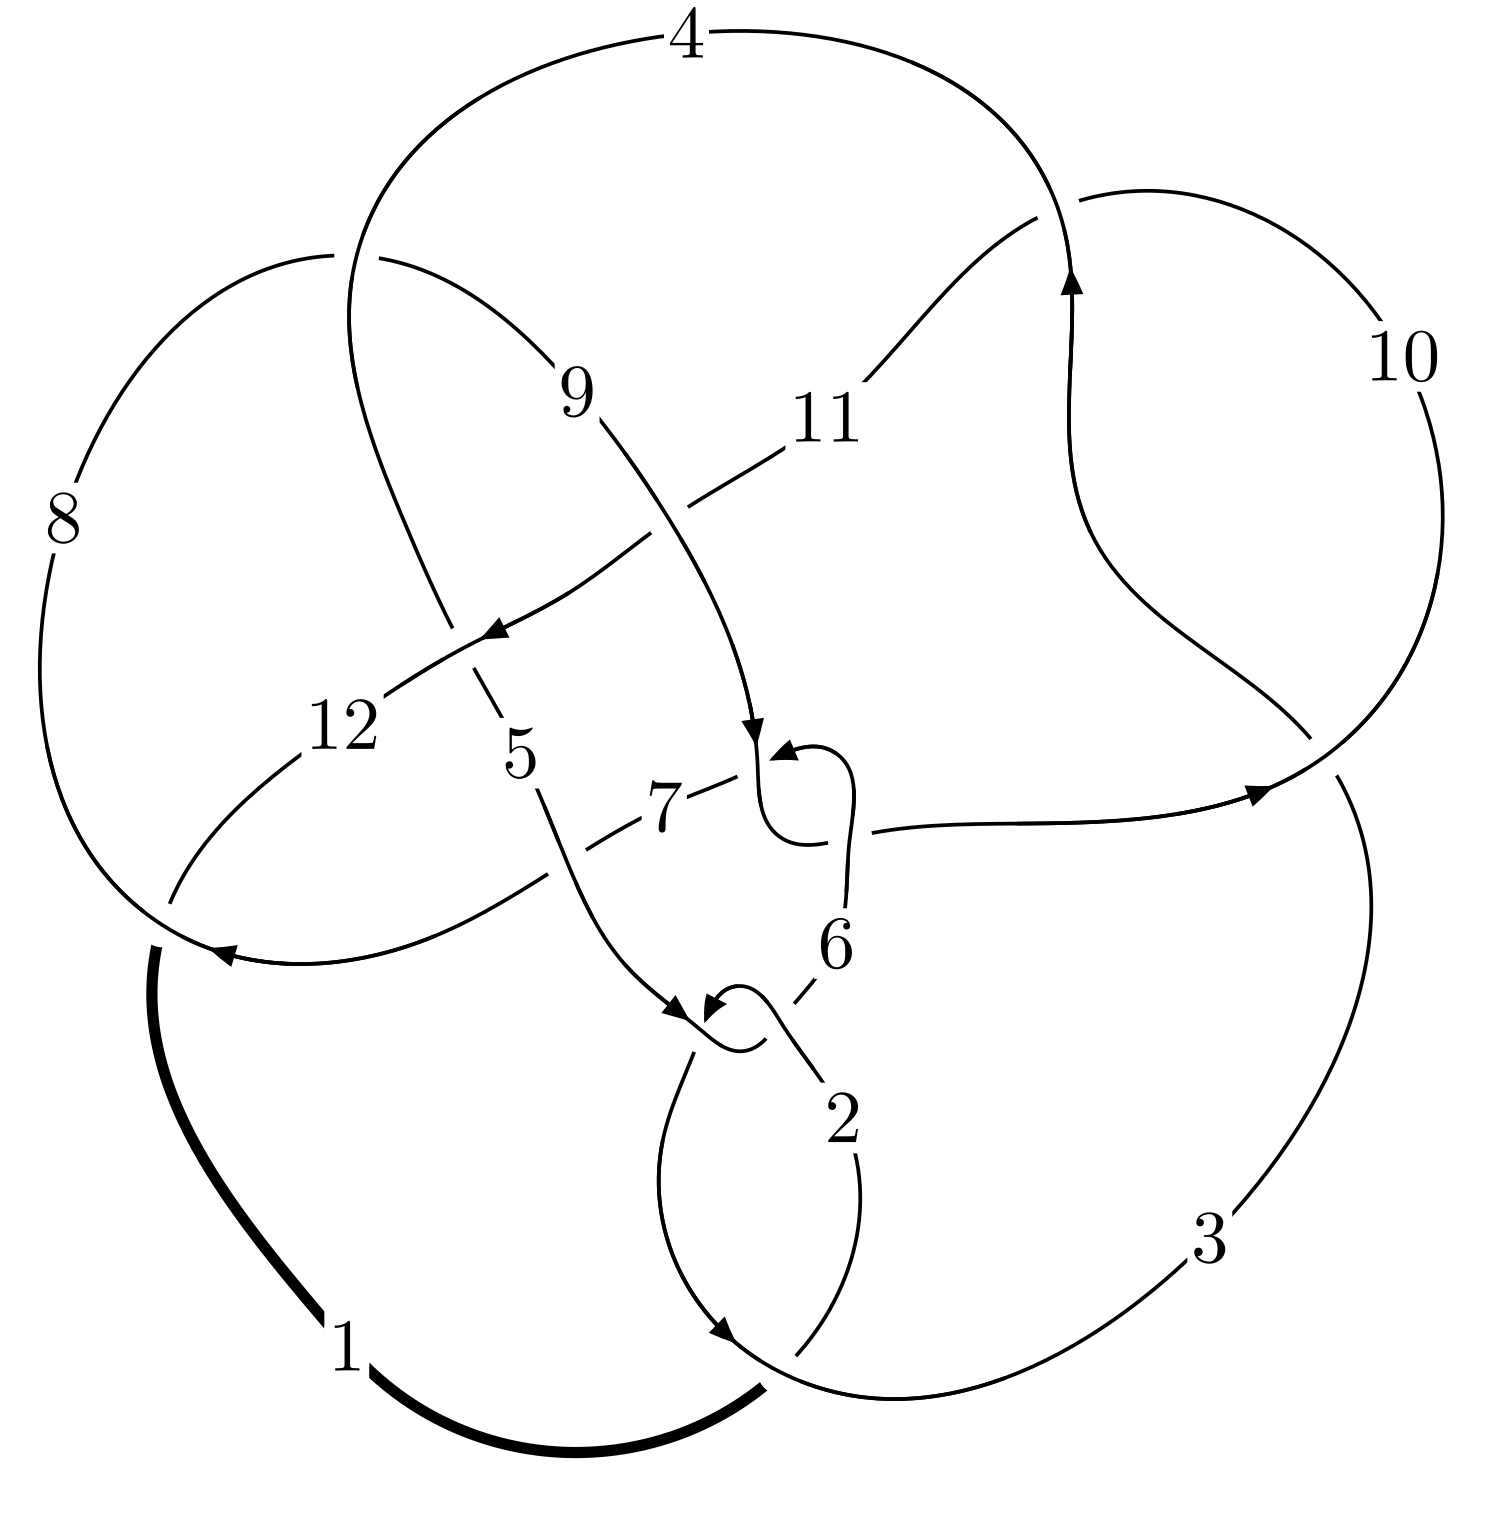
\includegraphics[width=112pt]{../../../GIT/diagram.site/Diagrams/png/2625_12n_0536.png}\\
\ \ \ A knot diagram\footnotemark}&
\allowdisplaybreaks
\textbf{Linearized knot diagam} \\
\cline{2-2}
 &
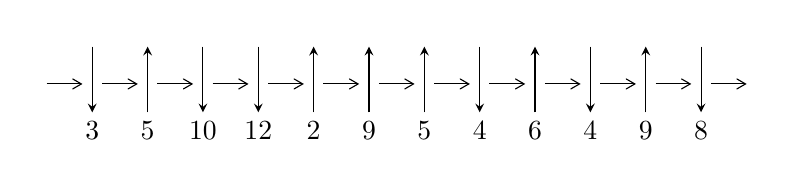
\begin{tikzpicture}[x=20pt, y=17pt]
	% nodes
	\node (C0) at (0, 0) {};
	\node (C1) at (1, 0) {};
	\node (C1U) at (1, +1) {};
	\node (C1D) at (1, -1) {3};

	\node (C2) at (2, 0) {};
	\node (C2U) at (2, +1) {};
	\node (C2D) at (2, -1) {5};

	\node (C3) at (3, 0) {};
	\node (C3U) at (3, +1) {};
	\node (C3D) at (3, -1) {10};

	\node (C4) at (4, 0) {};
	\node (C4U) at (4, +1) {};
	\node (C4D) at (4, -1) {12};

	\node (C5) at (5, 0) {};
	\node (C5U) at (5, +1) {};
	\node (C5D) at (5, -1) {2};

	\node (C6) at (6, 0) {};
	\node (C6U) at (6, +1) {};
	\node (C6D) at (6, -1) {9};

	\node (C7) at (7, 0) {};
	\node (C7U) at (7, +1) {};
	\node (C7D) at (7, -1) {5};

	\node (C8) at (8, 0) {};
	\node (C8U) at (8, +1) {};
	\node (C8D) at (8, -1) {4};

	\node (C9) at (9, 0) {};
	\node (C9U) at (9, +1) {};
	\node (C9D) at (9, -1) {6};

	\node (C10) at (10, 0) {};
	\node (C10U) at (10, +1) {};
	\node (C10D) at (10, -1) {4};

	\node (C11) at (11, 0) {};
	\node (C11U) at (11, +1) {};
	\node (C11D) at (11, -1) {9};

	\node (C12) at (12, 0) {};
	\node (C12U) at (12, +1) {};
	\node (C12D) at (12, -1) {8};
	\node (C13) at (13, 0) {};

	% arrows
	\draw[->,>={angle 60}]
	(C0) edge (C1) (C1) edge (C2) (C2) edge (C3) (C3) edge (C4) (C4) edge (C5) (C5) edge (C6) (C6) edge (C7) (C7) edge (C8) (C8) edge (C9) (C9) edge (C10) (C10) edge (C11) (C11) edge (C12) (C12) edge (C13) ;	\draw[->,>=stealth]
	(C1U) edge (C1D) (C2D) edge (C2U) (C3U) edge (C3D) (C4U) edge (C4D) (C5D) edge (C5U) (C6D) edge (C6U) (C7D) edge (C7U) (C8U) edge (C8D) (C9D) edge (C9U) (C10U) edge (C10D) (C11D) edge (C11U) (C12U) edge (C12D) ;
	\end{tikzpicture} \\
\hhline{~~} \\& 
\textbf{Solving Sequence} \\ \cline{2-2} 
 &
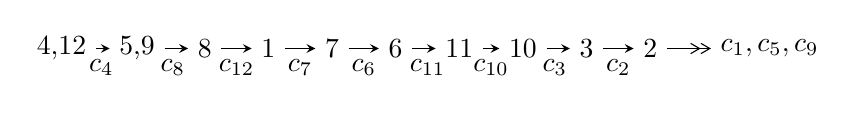
\begin{tikzpicture}[x=23pt, y=7pt]
	% node
	\node (A0) at (-1/8, 0) {4,12};
	\node (A1) at (17/16, 0) {5,9};
	\node (A2) at (17/8, 0) {8};
	\node (A3) at (25/8, 0) {1};
	\node (A4) at (33/8, 0) {7};
	\node (A5) at (41/8, 0) {6};
	\node (A6) at (49/8, 0) {11};
	\node (A7) at (57/8, 0) {10};
	\node (A8) at (65/8, 0) {3};
	\node (A9) at (73/8, 0) {2};
	\node (C1) at (1/2, -1) {$c_{4}$};
	\node (C2) at (13/8, -1) {$c_{8}$};
	\node (C3) at (21/8, -1) {$c_{12}$};
	\node (C4) at (29/8, -1) {$c_{7}$};
	\node (C5) at (37/8, -1) {$c_{6}$};
	\node (C6) at (45/8, -1) {$c_{11}$};
	\node (C7) at (53/8, -1) {$c_{10}$};
	\node (C8) at (61/8, -1) {$c_{3}$};
	\node (C9) at (69/8, -1) {$c_{2}$};
	\node (A10) at (11, 0) {$c_{1},c_{5},c_{9}$};

	% edge
	\draw[->,>=stealth]	
	(A0) edge (A1) (A1) edge (A2) (A2) edge (A3) (A3) edge (A4) (A4) edge (A5) (A5) edge (A6) (A6) edge (A7) (A7) edge (A8) (A8) edge (A9) ;
	\draw[->>,>={angle 60}]	
	(A9) edge (A10);
\end{tikzpicture} \\ 

\end{tabular} \\

\footnotetext{
The image of knot diagram is generated by the software ``\textbf{Draw programme}" developed by Andrew Bartholomew(\url{http://www.layer8.co.uk/maths/draw/index.htm\#Running-draw}), where we modified some parts for our purpose(\url{https://github.com/CATsTAILs/LinksPainter}).
}\phantom \\ \newline 
\centering \textbf{Ideals for irreducible components\footnotemark of $X_{\text{par}}$} 
 
\begin{align*}
I^u_{1}&=\langle 
1.71591\times10^{136} u^{61}+3.72192\times10^{136} u^{60}+\cdots+3.75605\times10^{136} b-9.70874\times10^{136},\\
\phantom{I^u_{1}}&\phantom{= \langle  }-7.27064\times10^{135} u^{61}-1.52290\times10^{136} u^{60}+\cdots+3.75605\times10^{136} a-1.84906\times10^{137},\\
\phantom{I^u_{1}}&\phantom{= \langle  }u^{62}+3 u^{61}+\cdots+6 u+1\rangle \\
I^u_{2}&=\langle 
163809549521227 u^{21}+58330736636863 u^{20}+\cdots+384149611137554 b+205005886037235,\\
\phantom{I^u_{2}}&\phantom{= \langle  }-51253454018903 u^{21}+148522476867159 u^{20}+\cdots+384149611137554 a-60479472657577,\\
\phantom{I^u_{2}}&\phantom{= \langle  }u^{22}-5 u^{20}+\cdots+2 u+1\rangle \\
\\
\end{align*}
\raggedright * 2 irreducible components of $\dim_{\mathbb{C}}=0$, with total 84 representations.\\
\footnotetext{All coefficients of polynomials are rational numbers. But the coefficients are sometimes approximated in decimal forms when there is not enough margin.}
\newpage
\renewcommand{\arraystretch}{1}
\centering \section*{I. $I^u_{1}= \langle 1.72\times10^{136} u^{61}+3.72\times10^{136} u^{60}+\cdots+3.76\times10^{136} b-9.71\times10^{136},\;-7.27\times10^{135} u^{61}-1.52\times10^{136} u^{60}+\cdots+3.76\times10^{136} a-1.85\times10^{137},\;u^{62}+3 u^{61}+\cdots+6 u+1 \rangle$}
\flushleft \textbf{(i) Arc colorings}\\
\begin{tabular}{m{7pt} m{180pt} m{7pt} m{180pt} }
\flushright $a_{4}=$&$\begin{pmatrix}1\\0\end{pmatrix}$ \\
\flushright $a_{12}=$&$\begin{pmatrix}0\\u\end{pmatrix}$ \\
\flushright $a_{5}=$&$\begin{pmatrix}1\\u^2\end{pmatrix}$ \\
\flushright $a_{9}=$&$\begin{pmatrix}0.193572 u^{61}+0.405454 u^{60}+\cdots+27.6970 u+4.92287\\-0.456839 u^{61}-0.990915 u^{60}+\cdots+18.2428 u+2.58483\end{pmatrix}$ \\
\flushright $a_{8}=$&$\begin{pmatrix}-0.263267 u^{61}-0.585461 u^{60}+\cdots+45.9398 u+7.50770\\-0.456839 u^{61}-0.990915 u^{60}+\cdots+18.2428 u+2.58483\end{pmatrix}$ \\
\flushright $a_{1}=$&$\begin{pmatrix}1.16917 u^{61}+3.24162 u^{60}+\cdots+20.2903 u+1.35776\\1.30286 u^{61}+4.60798 u^{60}+\cdots+14.7698 u+0.862367\end{pmatrix}$ \\
\flushright $a_{7}=$&$\begin{pmatrix}1.18336 u^{61}+3.73183 u^{60}+\cdots+26.7343 u+4.71853\\-1.32861 u^{61}-4.00841 u^{60}+\cdots+16.9317 u+2.60741\end{pmatrix}$ \\
\flushright $a_{6}=$&$\begin{pmatrix}2.34621 u^{61}+7.59680 u^{60}+\cdots+30.9047 u+3.59561\\1.43721 u^{61}+4.71130 u^{60}+\cdots+6.07767 u-0.182858\end{pmatrix}$ \\
\flushright $a_{11}=$&$\begin{pmatrix}-0.0591481 u^{61}-0.655677 u^{60}+\cdots+9.74878 u+1.14092\\-0.0745467 u^{61}-0.710685 u^{60}+\cdots-2.22824 u-0.645530\end{pmatrix}$ \\
\flushright $a_{10}=$&$\begin{pmatrix}-0.133695 u^{61}-1.36636 u^{60}+\cdots+7.52055 u+0.495394\\-0.0745467 u^{61}-0.710685 u^{60}+\cdots-2.22824 u-0.645530\end{pmatrix}$ \\
\flushright $a_{3}=$&$\begin{pmatrix}3.14078 u^{61}+9.08276 u^{60}+\cdots-3.04070 u+2.45575\\0.541059 u^{61}+1.40800 u^{60}+\cdots-0.406442 u+0.432472\end{pmatrix}$ \\
\flushright $a_{2}=$&$\begin{pmatrix}1.87526 u^{61}+5.39621 u^{60}+\cdots-3.73749 u+2.36287\\0.865858 u^{61}+2.48532 u^{60}+\cdots+0.198925 u+0.322445\end{pmatrix}$\\&\end{tabular}
\flushleft \textbf{(ii) Obstruction class $= -1$}\\~\\
\flushleft \textbf{(iii) Cusp Shapes $= -10.2334 u^{61}-37.5928 u^{60}+\cdots-136.983 u-17.5188$}\\~\\
\newpage\renewcommand{\arraystretch}{1}
\flushleft \textbf{(iv) u-Polynomials at the component}\newline \\
\begin{tabular}{m{50pt}|m{274pt}}
Crossings & \hspace{64pt}u-Polynomials at each crossing \\
\hline $$\begin{aligned}c_{1}\end{aligned}$$&$\begin{aligned}
&u^{62}+22 u^{61}+\cdots+620 u+4
\end{aligned}$\\
\hline $$\begin{aligned}c_{2},c_{5}\end{aligned}$$&$\begin{aligned}
&u^{62}+11 u^{60}+\cdots-10 u+2
\end{aligned}$\\
\hline $$\begin{aligned}c_{3},c_{10}\end{aligned}$$&$\begin{aligned}
&u^{62}+u^{61}+\cdots+170 u+289
\end{aligned}$\\
\hline $$\begin{aligned}c_{4}\end{aligned}$$&$\begin{aligned}
&u^{62}+3 u^{61}+\cdots+6 u+1
\end{aligned}$\\
\hline $$\begin{aligned}c_{6},c_{9}\end{aligned}$$&$\begin{aligned}
&u^{62}+2 u^{61}+\cdots+10 u+1
\end{aligned}$\\
\hline $$\begin{aligned}c_{7}\end{aligned}$$&$\begin{aligned}
&u^{62}+8 u^{61}+\cdots-12576553 u+1906367
\end{aligned}$\\
\hline $$\begin{aligned}c_{8}\end{aligned}$$&$\begin{aligned}
&u^{62}+2 u^{61}+\cdots-68 u+26
\end{aligned}$\\
\hline $$\begin{aligned}c_{11}\end{aligned}$$&$\begin{aligned}
&u^{62}- u^{61}+\cdots-150 u+67
\end{aligned}$\\
\hline $$\begin{aligned}c_{12}\end{aligned}$$&$\begin{aligned}
&u^{62}- u^{61}+\cdots-104469 u+9059
\end{aligned}$\\
\hline
\end{tabular}\\~\\
\newpage\renewcommand{\arraystretch}{1}
\flushleft \textbf{(v) Riley Polynomials at the component}\newline \\
\begin{tabular}{m{50pt}|m{274pt}}
Crossings & \hspace{64pt}Riley Polynomials at each crossing \\
\hline $$\begin{aligned}c_{1}\end{aligned}$$&$\begin{aligned}
&y^{62}+46 y^{61}+\cdots-67792 y+16
\end{aligned}$\\
\hline $$\begin{aligned}c_{2},c_{5}\end{aligned}$$&$\begin{aligned}
&y^{62}+22 y^{61}+\cdots+620 y+4
\end{aligned}$\\
\hline $$\begin{aligned}c_{3},c_{10}\end{aligned}$$&$\begin{aligned}
&y^{62}- y^{61}+\cdots+2388874 y+83521
\end{aligned}$\\
\hline $$\begin{aligned}c_{4}\end{aligned}$$&$\begin{aligned}
&y^{62}-5 y^{61}+\cdots+14 y+1
\end{aligned}$\\
\hline $$\begin{aligned}c_{6},c_{9}\end{aligned}$$&$\begin{aligned}
&y^{62}+12 y^{61}+\cdots+52 y+1
\end{aligned}$\\
\hline $$\begin{aligned}c_{7}\end{aligned}$$&$\begin{aligned}
&y^{62}-84 y^{61}+\cdots-322575225344421 y+3634235138689
\end{aligned}$\\
\hline $$\begin{aligned}c_{8}\end{aligned}$$&$\begin{aligned}
&y^{62}+56 y^{61}+\cdots-22200 y+676
\end{aligned}$\\
\hline $$\begin{aligned}c_{11}\end{aligned}$$&$\begin{aligned}
&y^{62}-59 y^{61}+\cdots+164028 y+4489
\end{aligned}$\\
\hline $$\begin{aligned}c_{12}\end{aligned}$$&$\begin{aligned}
&y^{62}+67 y^{61}+\cdots+488736985 y+82065481
\end{aligned}$\\
\hline
\end{tabular}\\~\\
\newpage\flushleft \textbf{(vi) Complex Volumes and Cusp Shapes}
$$\begin{array}{c|c|c}  
\text{Solutions to }I^u_{1}& \I (\text{vol} + \sqrt{-1}CS) & \text{Cusp shape}\\
 \hline 
\begin{aligned}
u &= \phantom{-}0.165930 + 0.930592 I \\
a &= -0.10701 + 2.06026 I \\
b &= -0.057682 - 0.972148 I\end{aligned}
 & \phantom{-}3.40685 - 2.08743 I & \phantom{-}8.13116 + 4.36654 I \\ \hline\begin{aligned}
u &= \phantom{-}0.165930 - 0.930592 I \\
a &= -0.10701 - 2.06026 I \\
b &= -0.057682 + 0.972148 I\end{aligned}
 & \phantom{-}3.40685 + 2.08743 I & \phantom{-}8.13116 - 4.36654 I \\ \hline\begin{aligned}
u &= -0.997985 + 0.380629 I \\
a &= \phantom{-}0.433419 + 1.028500 I \\
b &= -0.13150 - 1.44905 I\end{aligned}
 & -1.18532 + 5.73345 I & \phantom{-0.000000 } 0. - 8.28149 I \\ \hline\begin{aligned}
u &= -0.997985 - 0.380629 I \\
a &= \phantom{-}0.433419 - 1.028500 I \\
b &= -0.13150 + 1.44905 I\end{aligned}
 & -1.18532 - 5.73345 I & \phantom{-0.000000 -}0. + 8.28149 I \\ \hline\begin{aligned}
u &= -0.002944 + 0.924364 I \\
a &= \phantom{-}0.211183 - 1.006820 I \\
b &= -0.16712 + 1.85863 I\end{aligned}
 & \phantom{-}2.71444 + 3.86842 I & \phantom{-}6.79055 - 7.43016 I \\ \hline\begin{aligned}
u &= -0.002944 - 0.924364 I \\
a &= \phantom{-}0.211183 + 1.006820 I \\
b &= -0.16712 - 1.85863 I\end{aligned}
 & \phantom{-}2.71444 - 3.86842 I & \phantom{-}6.79055 + 7.43016 I \\ \hline\begin{aligned}
u &= -0.812041 + 0.713431 I \\
a &= -0.915182 - 0.646168 I \\
b &= -0.609084 + 0.870903 I\end{aligned}
 & -0.67509 + 1.55554 I & \phantom{-0.000000 } 0 \\ \hline\begin{aligned}
u &= -0.812041 - 0.713431 I \\
a &= -0.915182 + 0.646168 I \\
b &= -0.609084 - 0.870903 I\end{aligned}
 & -0.67509 - 1.55554 I & \phantom{-0.000000 } 0 \\ \hline\begin{aligned}
u &= -1.063550 + 0.207154 I \\
a &= -0.420018 + 0.637174 I \\
b &= \phantom{-}0.467651 + 0.802572 I\end{aligned}
 & -5.03634 - 0.65577 I & \phantom{-0.000000 } 0 \\ \hline\begin{aligned}
u &= -1.063550 - 0.207154 I \\
a &= -0.420018 - 0.637174 I \\
b &= \phantom{-}0.467651 - 0.802572 I\end{aligned}
 & -5.03634 + 0.65577 I & \phantom{-0.000000 } 0\\
 \hline 
 \end{array}$$\newpage$$\begin{array}{c|c|c}  
\text{Solutions to }I^u_{1}& \I (\text{vol} + \sqrt{-1}CS) & \text{Cusp shape}\\
 \hline 
\begin{aligned}
u &= -0.465488 + 0.779154 I \\
a &= -0.092600 - 1.357340 I \\
b &= -0.97065 + 1.22533 I\end{aligned}
 & -2.61957 + 4.38386 I & \phantom{-}1.07305 - 7.42421 I \\ \hline\begin{aligned}
u &= -0.465488 - 0.779154 I \\
a &= -0.092600 + 1.357340 I \\
b &= -0.97065 - 1.22533 I\end{aligned}
 & -2.61957 - 4.38386 I & \phantom{-}1.07305 + 7.42421 I \\ \hline\begin{aligned}
u &= \phantom{-}0.750587 + 0.427782 I \\
a &= \phantom{-}1.65282 - 0.94218 I \\
b &= \phantom{-}0.736969 + 0.934309 I\end{aligned}
 & -0.11147 - 6.99469 I & -3.20173 + 9.81711 I \\ \hline\begin{aligned}
u &= \phantom{-}0.750587 - 0.427782 I \\
a &= \phantom{-}1.65282 + 0.94218 I \\
b &= \phantom{-}0.736969 - 0.934309 I\end{aligned}
 & -0.11147 + 6.99469 I & -3.20173 - 9.81711 I \\ \hline\begin{aligned}
u &= \phantom{-}1.221520 + 0.120806 I \\
a &= \phantom{-}0.339911 - 0.433001 I \\
b &= -0.558973 - 0.091877 I\end{aligned}
 & -7.45390 - 2.15136 I & \phantom{-0.000000 } 0 \\ \hline\begin{aligned}
u &= \phantom{-}1.221520 - 0.120806 I \\
a &= \phantom{-}0.339911 + 0.433001 I \\
b &= -0.558973 + 0.091877 I\end{aligned}
 & -7.45390 + 2.15136 I & \phantom{-0.000000 } 0 \\ \hline\begin{aligned}
u &= -0.517704 + 0.562485 I \\
a &= -0.668372 - 0.070624 I \\
b &= -0.476542 + 0.257017 I\end{aligned}
 & -1.05258 + 1.18693 I & -4.45668 - 4.18814 I \\ \hline\begin{aligned}
u &= -0.517704 - 0.562485 I \\
a &= -0.668372 + 0.070624 I \\
b &= -0.476542 - 0.257017 I\end{aligned}
 & -1.05258 - 1.18693 I & -4.45668 + 4.18814 I \\ \hline\begin{aligned}
u &= \phantom{-}0.523431 + 0.513052 I \\
a &= -0.535706 + 1.288960 I \\
b &= \phantom{-}0.266709 - 1.273450 I\end{aligned}
 & \phantom{-}1.82519 - 1.36296 I & \phantom{-}1.54329 + 4.17454 I \\ \hline\begin{aligned}
u &= \phantom{-}0.523431 - 0.513052 I \\
a &= -0.535706 - 1.288960 I \\
b &= \phantom{-}0.266709 + 1.273450 I\end{aligned}
 & \phantom{-}1.82519 + 1.36296 I & \phantom{-}1.54329 - 4.17454 I\\
 \hline 
 \end{array}$$\newpage$$\begin{array}{c|c|c}  
\text{Solutions to }I^u_{1}& \I (\text{vol} + \sqrt{-1}CS) & \text{Cusp shape}\\
 \hline 
\begin{aligned}
u &= \phantom{-}0.321102 + 0.647348 I \\
a &= -0.022673 + 1.348950 I \\
b &= \phantom{-}0.501475 - 0.865448 I\end{aligned}
 & \phantom{-}1.85599 - 1.13423 I & -0.309363 - 0.900307 I \\ \hline\begin{aligned}
u &= \phantom{-}0.321102 - 0.647348 I \\
a &= -0.022673 - 1.348950 I \\
b &= \phantom{-}0.501475 + 0.865448 I\end{aligned}
 & \phantom{-}1.85599 + 1.13423 I & -0.309363 + 0.900307 I \\ \hline\begin{aligned}
u &= -0.168667 + 0.660664 I \\
a &= -3.06985 + 0.38017 I \\
b &= \phantom{-}0.171594 + 0.004198 I\end{aligned}
 & \phantom{-}2.65932 + 6.57779 I & \phantom{-}7.85703 - 7.89113 I \\ \hline\begin{aligned}
u &= -0.168667 - 0.660664 I \\
a &= -3.06985 - 0.38017 I \\
b &= \phantom{-}0.171594 - 0.004198 I\end{aligned}
 & \phantom{-}2.65932 - 6.57779 I & \phantom{-}7.85703 + 7.89113 I \\ \hline\begin{aligned}
u &= -1.315760 + 0.177104 I \\
a &= -0.421905 + 0.140944 I \\
b &= -0.418914 + 0.165670 I\end{aligned}
 & -2.41902 + 0.19351 I & \phantom{-0.000000 } 0 \\ \hline\begin{aligned}
u &= -1.315760 - 0.177104 I \\
a &= -0.421905 - 0.140944 I \\
b &= -0.418914 - 0.165670 I\end{aligned}
 & -2.41902 - 0.19351 I & \phantom{-0.000000 } 0 \\ \hline\begin{aligned}
u &= \phantom{-}0.234273 + 0.612614 I \\
a &= \phantom{-}2.46365 + 1.67487 I \\
b &= -0.105327 - 0.177690 I\end{aligned}
 & \phantom{-}3.58080 - 1.15954 I & \phantom{-}9.57507 + 5.43915 I \\ \hline\begin{aligned}
u &= \phantom{-}0.234273 - 0.612614 I \\
a &= \phantom{-}2.46365 - 1.67487 I \\
b &= -0.105327 + 0.177690 I\end{aligned}
 & \phantom{-}3.58080 + 1.15954 I & \phantom{-}9.57507 - 5.43915 I \\ \hline\begin{aligned}
u &= -0.904086 + 1.045360 I \\
a &= -0.249561 - 0.737893 I \\
b &= -0.42512 + 1.73156 I\end{aligned}
 & -0.00214 + 4.68956 I & \phantom{-0.000000 } 0 \\ \hline\begin{aligned}
u &= -0.904086 - 1.045360 I \\
a &= -0.249561 + 0.737893 I \\
b &= -0.42512 - 1.73156 I\end{aligned}
 & -0.00214 - 4.68956 I & \phantom{-0.000000 } 0\\
 \hline 
 \end{array}$$\newpage$$\begin{array}{c|c|c}  
\text{Solutions to }I^u_{1}& \I (\text{vol} + \sqrt{-1}CS) & \text{Cusp shape}\\
 \hline 
\begin{aligned}
u &= \phantom{-}0.281954 + 0.542697 I \\
a &= \phantom{-}0.219911 + 0.087140 I \\
b &= -2.26522 - 0.10868 I\end{aligned}
 & \phantom{-}2.06711 - 7.02714 I & \phantom{-}7.2802 + 14.8527 I \\ \hline\begin{aligned}
u &= \phantom{-}0.281954 - 0.542697 I \\
a &= \phantom{-}0.219911 - 0.087140 I \\
b &= -2.26522 + 0.10868 I\end{aligned}
 & \phantom{-}2.06711 + 7.02714 I & \phantom{-}7.2802 - 14.8527 I \\ \hline\begin{aligned}
u &= -0.026975 + 0.606723 I \\
a &= -0.084880 + 0.310459 I \\
b &= \phantom{-}1.89438 + 0.04499 I\end{aligned}
 & \phantom{-}3.66976 + 0.24782 I & \phantom{-}12.04590 + 2.79775 I \\ \hline\begin{aligned}
u &= -0.026975 - 0.606723 I \\
a &= -0.084880 - 0.310459 I \\
b &= \phantom{-}1.89438 - 0.04499 I\end{aligned}
 & \phantom{-}3.66976 - 0.24782 I & \phantom{-}12.04590 - 2.79775 I \\ \hline\begin{aligned}
u &= \phantom{-}0.335377 + 0.481418 I \\
a &= -0.06783 - 2.73237 I \\
b &= \phantom{-}0.557255 + 1.037380 I\end{aligned}
 & -4.01107 - 3.42086 I & -8.07352 + 4.07528 I \\ \hline\begin{aligned}
u &= \phantom{-}0.335377 - 0.481418 I \\
a &= -0.06783 + 2.73237 I \\
b &= \phantom{-}0.557255 - 1.037380 I\end{aligned}
 & -4.01107 + 3.42086 I & -8.07352 - 4.07528 I \\ \hline\begin{aligned}
u &= \phantom{-}0.92096 + 1.12984 I \\
a &= -0.401949 + 1.176920 I \\
b &= -0.52928 - 1.72739 I\end{aligned}
 & \phantom{-}9.40777 - 1.77606 I & \phantom{-0.000000 } 0 \\ \hline\begin{aligned}
u &= \phantom{-}0.92096 - 1.12984 I \\
a &= -0.401949 - 1.176920 I \\
b &= -0.52928 + 1.72739 I\end{aligned}
 & \phantom{-}9.40777 + 1.77606 I & \phantom{-0.000000 } 0 \\ \hline\begin{aligned}
u &= -0.93058 + 1.15260 I \\
a &= \phantom{-}0.366572 + 1.172380 I \\
b &= \phantom{-}0.68767 - 1.60197 I\end{aligned}
 & \phantom{-}9.16673 + 8.01243 I & \phantom{-0.000000 } 0 \\ \hline\begin{aligned}
u &= -0.93058 - 1.15260 I \\
a &= \phantom{-}0.366572 - 1.172380 I \\
b &= \phantom{-}0.68767 + 1.60197 I\end{aligned}
 & \phantom{-}9.16673 - 8.01243 I & \phantom{-0.000000 } 0\\
 \hline 
 \end{array}$$\newpage$$\begin{array}{c|c|c}  
\text{Solutions to }I^u_{1}& \I (\text{vol} + \sqrt{-1}CS) & \text{Cusp shape}\\
 \hline 
\begin{aligned}
u &= \phantom{-}1.01454 + 1.08458 I \\
a &= -0.612869 + 1.143460 I \\
b &= -0.227460 - 1.383390 I\end{aligned}
 & \phantom{-}4.02353 - 3.94644 I & \phantom{-0.000000 } 0 \\ \hline\begin{aligned}
u &= \phantom{-}1.01454 - 1.08458 I \\
a &= -0.612869 - 1.143460 I \\
b &= -0.227460 + 1.383390 I\end{aligned}
 & \phantom{-}4.02353 + 3.94644 I & \phantom{-0.000000 } 0 \\ \hline\begin{aligned}
u &= \phantom{-}1.45278 + 0.32226 I \\
a &= \phantom{-}0.186002 + 0.283851 I \\
b &= \phantom{-}0.180304 - 0.249974 I\end{aligned}
 & -5.07079 - 5.71196 I & \phantom{-0.000000 } 0 \\ \hline\begin{aligned}
u &= \phantom{-}1.45278 - 0.32226 I \\
a &= \phantom{-}0.186002 - 0.283851 I \\
b &= \phantom{-}0.180304 + 0.249974 I\end{aligned}
 & -5.07079 + 5.71196 I & \phantom{-0.000000 } 0 \\ \hline\begin{aligned}
u &= -0.172079 + 0.459052 I \\
a &= -0.346327 + 1.016920 I \\
b &= \phantom{-}0.095770 + 0.617374 I\end{aligned}
 & -0.26698 + 2.11215 I & -2.44927 - 3.44810 I \\ \hline\begin{aligned}
u &= -0.172079 - 0.459052 I \\
a &= -0.346327 - 1.016920 I \\
b &= \phantom{-}0.095770 - 0.617374 I\end{aligned}
 & -0.26698 - 2.11215 I & -2.44927 + 3.44810 I \\ \hline\begin{aligned}
u &= \phantom{-}1.16422 + 0.97896 I \\
a &= -0.845511 + 0.676945 I \\
b &= -0.00205 - 1.54662 I\end{aligned}
 & \phantom{-}8.59237 - 5.95049 I & \phantom{-0.000000 } 0 \\ \hline\begin{aligned}
u &= \phantom{-}1.16422 - 0.97896 I \\
a &= -0.845511 - 0.676945 I \\
b &= -0.00205 + 1.54662 I\end{aligned}
 & \phantom{-}8.59237 + 5.95049 I & \phantom{-0.000000 } 0 \\ \hline\begin{aligned}
u &= \phantom{-}1.09741 + 1.08495 I \\
a &= \phantom{-}0.471415 - 1.019370 I \\
b &= \phantom{-}0.60017 + 1.72962 I\end{aligned}
 & \phantom{-}9.91197 - 8.88268 I & \phantom{-0.000000 } 0 \\ \hline\begin{aligned}
u &= \phantom{-}1.09741 - 1.08495 I \\
a &= \phantom{-}0.471415 + 1.019370 I \\
b &= \phantom{-}0.60017 - 1.72962 I\end{aligned}
 & \phantom{-}9.91197 + 8.88268 I & \phantom{-0.000000 } 0\\
 \hline 
 \end{array}$$\newpage$$\begin{array}{c|c|c}  
\text{Solutions to }I^u_{1}& \I (\text{vol} + \sqrt{-1}CS) & \text{Cusp shape}\\
 \hline 
\begin{aligned}
u &= -1.10944 + 1.08719 I \\
a &= -0.451584 - 1.116400 I \\
b &= -0.68155 + 1.68234 I\end{aligned}
 & \phantom{-}8.0311 + 16.0146 I & \phantom{-0.000000 } 0 \\ \hline\begin{aligned}
u &= -1.10944 - 1.08719 I \\
a &= -0.451584 + 1.116400 I \\
b &= -0.68155 - 1.68234 I\end{aligned}
 & \phantom{-}8.0311 - 16.0146 I & \phantom{-0.000000 } 0 \\ \hline\begin{aligned}
u &= \phantom{-}1.04855 + 1.15112 I \\
a &= \phantom{-}0.698585 - 0.718469 I \\
b &= \phantom{-}0.06404 + 1.56751 I\end{aligned}
 & \phantom{-}10.11830 + 0.77137 I & \phantom{-0.000000 } 0 \\ \hline\begin{aligned}
u &= \phantom{-}1.04855 - 1.15112 I \\
a &= \phantom{-}0.698585 + 0.718469 I \\
b &= \phantom{-}0.06404 - 1.56751 I\end{aligned}
 & \phantom{-}10.11830 - 0.77137 I & \phantom{-0.000000 } 0 \\ \hline\begin{aligned}
u &= -1.20685 + 0.99490 I \\
a &= \phantom{-}0.725567 + 0.568353 I \\
b &= -0.13679 - 1.45257 I\end{aligned}
 & \phantom{-}8.26868 - 0.11939 I & \phantom{-0.000000 } 0 \\ \hline\begin{aligned}
u &= -1.20685 - 0.99490 I \\
a &= \phantom{-}0.725567 - 0.568353 I \\
b &= -0.13679 + 1.45257 I\end{aligned}
 & \phantom{-}8.26868 + 0.11939 I & \phantom{-0.000000 } 0 \\ \hline\begin{aligned}
u &= -1.05420 + 1.18099 I \\
a &= -0.710445 - 0.706964 I \\
b &= \phantom{-}0.12015 + 1.50569 I\end{aligned}
 & \phantom{-}8.28897 - 7.80965 I & \phantom{-0.000000 } 0 \\ \hline\begin{aligned}
u &= -1.05420 - 1.18099 I \\
a &= -0.710445 + 0.706964 I \\
b &= \phantom{-}0.12015 - 1.50569 I\end{aligned}
 & \phantom{-}8.28897 + 7.80965 I & \phantom{-0.000000 } 0 \\ \hline\begin{aligned}
u &= -1.08118 + 1.18882 I \\
a &= \phantom{-}0.421669 + 0.935093 I \\
b &= \phantom{-}0.258643 - 1.207240 I\end{aligned}
 & \phantom{-}3.27959 + 4.26299 I & \phantom{-0.000000 } 0 \\ \hline\begin{aligned}
u &= -1.08118 - 1.18882 I \\
a &= \phantom{-}0.421669 - 0.935093 I \\
b &= \phantom{-}0.258643 + 1.207240 I\end{aligned}
 & \phantom{-}3.27959 - 4.26299 I & \phantom{-0.000000 } 0\\
 \hline 
 \end{array}$$\newpage$$\begin{array}{c|c|c}  
\text{Solutions to }I^u_{1}& \I (\text{vol} + \sqrt{-1}CS) & \text{Cusp shape}\\
 \hline 
\begin{aligned}
u &= -0.203127 + 0.142996 I \\
a &= \phantom{-}1.83356 + 2.81105 I \\
b &= \phantom{-}0.160472 + 0.965429 I\end{aligned}
 & -0.23208 + 2.09229 I & -2.77990 - 2.89354 I \\ \hline\begin{aligned}
u &= -0.203127 - 0.142996 I \\
a &= \phantom{-}1.83356 - 2.81105 I \\
b &= \phantom{-}0.160472 - 0.965429 I\end{aligned}
 & -0.23208 - 2.09229 I & -2.77990 + 2.89354 I\\
 \hline 
 \end{array}$$\newpage\newpage\renewcommand{\arraystretch}{1}
\centering \section*{II. $I^u_{2}= \langle 1.64\times10^{14} u^{21}+5.83\times10^{13} u^{20}+\cdots+3.84\times10^{14} b+2.05\times10^{14},\;-5.13\times10^{13} u^{21}+1.49\times10^{14} u^{20}+\cdots+3.84\times10^{14} a-6.05\times10^{13},\;u^{22}-5 u^{20}+\cdots+2 u+1 \rangle$}
\flushleft \textbf{(i) Arc colorings}\\
\begin{tabular}{m{7pt} m{180pt} m{7pt} m{180pt} }
\flushright $a_{4}=$&$\begin{pmatrix}1\\0\end{pmatrix}$ \\
\flushright $a_{12}=$&$\begin{pmatrix}0\\u\end{pmatrix}$ \\
\flushright $a_{5}=$&$\begin{pmatrix}1\\u^2\end{pmatrix}$ \\
\flushright $a_{9}=$&$\begin{pmatrix}0.133421 u^{21}-0.386627 u^{20}+\cdots+2.14873 u+0.157437\\-0.426421 u^{21}-0.151844 u^{20}+\cdots-0.826693 u-0.533662\end{pmatrix}$ \\
\flushright $a_{8}=$&$\begin{pmatrix}-0.293001 u^{21}-0.538470 u^{20}+\cdots+1.32204 u-0.376224\\-0.426421 u^{21}-0.151844 u^{20}+\cdots-0.826693 u-0.533662\end{pmatrix}$ \\
\flushright $a_{1}=$&$\begin{pmatrix}-0.647220 u^{21}-0.166162 u^{20}+\cdots-12.1300 u-4.73495\\-0.353043 u^{21}+0.155220 u^{20}+\cdots-3.80337 u-0.927868\end{pmatrix}$ \\
\flushright $a_{7}=$&$\begin{pmatrix}0.353956 u^{21}-0.383250 u^{20}+\cdots+3.51867 u+0.695908\\-0.552635 u^{21}-0.137768 u^{20}+\cdots-1.78409 u-0.688882\end{pmatrix}$ \\
\flushright $a_{6}=$&$\begin{pmatrix}0.342136 u^{21}+0.492525 u^{20}+\cdots+7.17325 u+3.00994\\0.162285 u^{21}-0.0994937 u^{20}+\cdots+2.68471 u+0.397069\end{pmatrix}$ \\
\flushright $a_{11}=$&$\begin{pmatrix}-0.00909788 u^{21}-0.359656 u^{20}+\cdots-3.79539 u-2.89303\\-0.285080 u^{21}+0.0382739 u^{20}+\cdots-2.53120 u-0.914050\end{pmatrix}$ \\
\flushright $a_{10}=$&$\begin{pmatrix}-0.294178 u^{21}-0.321382 u^{20}+\cdots-6.32659 u-3.80708\\-0.285080 u^{21}+0.0382739 u^{20}+\cdots-2.53120 u-0.914050\end{pmatrix}$ \\
\flushright $a_{3}=$&$\begin{pmatrix}-1.37389 u^{21}+0.229452 u^{20}+\cdots-7.40788 u-0.433030\\-0.527423 u^{21}+0.262335 u^{20}+\cdots-1.88437 u-0.163479\end{pmatrix}$ \\
\flushright $a_{2}=$&$\begin{pmatrix}-1.07248 u^{21}+0.185019 u^{20}+\cdots-4.60852 u-0.499002\\-0.522187 u^{21}+0.314870 u^{20}+\cdots-2.09691 u-0.119046\end{pmatrix}$\\&\end{tabular}
\flushleft \textbf{(ii) Obstruction class $= 1$}\\~\\
\flushleft \textbf{(iii) Cusp Shapes $= \frac{44792649864550}{192074805568777} u^{21}+\frac{164302245595680}{192074805568777} u^{20}+\cdots+\frac{1491146875316471}{192074805568777} u+\frac{304827721883127}{192074805568777}$}\\~\\
\newpage\renewcommand{\arraystretch}{1}
\flushleft \textbf{(iv) u-Polynomials at the component}\newline \\
\begin{tabular}{m{50pt}|m{274pt}}
Crossings & \hspace{64pt}u-Polynomials at each crossing \\
\hline $$\begin{aligned}c_{1}\end{aligned}$$&$\begin{aligned}
&u^{22}-13 u^{21}+\cdots-56 u+4
\end{aligned}$\\
\hline $$\begin{aligned}c_{2}\end{aligned}$$&$\begin{aligned}
&u^{22}+u^{21}+\cdots+2 u+2
\end{aligned}$\\
\hline $$\begin{aligned}c_{3}\end{aligned}$$&$\begin{aligned}
&u^{22}+2 u^{21}+\cdots+8 u+1
\end{aligned}$\\
\hline $$\begin{aligned}c_{4}\end{aligned}$$&$\begin{aligned}
&u^{22}-5 u^{20}+\cdots+2 u+1
\end{aligned}$\\
\hline $$\begin{aligned}c_{5}\end{aligned}$$&$\begin{aligned}
&u^{22}- u^{21}+\cdots-2 u+2
\end{aligned}$\\
\hline $$\begin{aligned}c_{6}\end{aligned}$$&$\begin{aligned}
&u^{22}+9 u^{21}+\cdots+4 u+1
\end{aligned}$\\
\hline $$\begin{aligned}c_{7}\end{aligned}$$&$\begin{aligned}
&u^{22}+u^{21}+\cdots+u+1
\end{aligned}$\\
\hline $$\begin{aligned}c_{8}\end{aligned}$$&$\begin{aligned}
&u^{22}+u^{21}+\cdots+9 u^2+2
\end{aligned}$\\
\hline $$\begin{aligned}c_{9}\end{aligned}$$&$\begin{aligned}
&u^{22}-9 u^{21}+\cdots-4 u+1
\end{aligned}$\\
\hline $$\begin{aligned}c_{10}\end{aligned}$$&$\begin{aligned}
&u^{22}-2 u^{21}+\cdots-8 u+1
\end{aligned}$\\
\hline $$\begin{aligned}c_{11}\end{aligned}$$&$\begin{aligned}
&u^{22}-2 u^{21}+\cdots-4 u+1
\end{aligned}$\\
\hline $$\begin{aligned}c_{12}\end{aligned}$$&$\begin{aligned}
&u^{22}+7 u^{20}+\cdots-3 u+1
\end{aligned}$\\
\hline
\end{tabular}\\~\\
\newpage\renewcommand{\arraystretch}{1}
\flushleft \textbf{(v) Riley Polynomials at the component}\newline \\
\begin{tabular}{m{50pt}|m{274pt}}
Crossings & \hspace{64pt}Riley Polynomials at each crossing \\
\hline $$\begin{aligned}c_{1}\end{aligned}$$&$\begin{aligned}
&y^{22}+y^{21}+\cdots-120 y+16
\end{aligned}$\\
\hline $$\begin{aligned}c_{2},c_{5}\end{aligned}$$&$\begin{aligned}
&y^{22}+13 y^{21}+\cdots+56 y+4
\end{aligned}$\\
\hline $$\begin{aligned}c_{3},c_{10}\end{aligned}$$&$\begin{aligned}
&y^{22}-18 y^{21}+\cdots-22 y+1
\end{aligned}$\\
\hline $$\begin{aligned}c_{4}\end{aligned}$$&$\begin{aligned}
&y^{22}-10 y^{21}+\cdots+10 y+1
\end{aligned}$\\
\hline $$\begin{aligned}c_{6},c_{9}\end{aligned}$$&$\begin{aligned}
&y^{22}+11 y^{21}+\cdots+12 y+1
\end{aligned}$\\
\hline $$\begin{aligned}c_{7}\end{aligned}$$&$\begin{aligned}
&y^{22}-13 y^{21}+\cdots+3 y+1
\end{aligned}$\\
\hline $$\begin{aligned}c_{8}\end{aligned}$$&$\begin{aligned}
&y^{22}+11 y^{21}+\cdots+36 y+4
\end{aligned}$\\
\hline $$\begin{aligned}c_{11}\end{aligned}$$&$\begin{aligned}
&y^{22}-12 y^{21}+\cdots-8 y+1
\end{aligned}$\\
\hline $$\begin{aligned}c_{12}\end{aligned}$$&$\begin{aligned}
&y^{22}+14 y^{21}+\cdots+17 y+1
\end{aligned}$\\
\hline
\end{tabular}\\~\\
\newpage\flushleft \textbf{(vi) Complex Volumes and Cusp Shapes}
$$\begin{array}{c|c|c}  
\text{Solutions to }I^u_{2}& \I (\text{vol} + \sqrt{-1}CS) & \text{Cusp shape}\\
 \hline 
\begin{aligned}
u &= -0.730385 + 0.664526 I \\
a &= -0.119371 - 1.335790 I \\
b &= -0.70021 + 1.27249 I\end{aligned}
 & -4.10993 + 5.20936 I & -6.16659 - 7.45799 I \\ \hline\begin{aligned}
u &= -0.730385 - 0.664526 I \\
a &= -0.119371 + 1.335790 I \\
b &= -0.70021 - 1.27249 I\end{aligned}
 & -4.10993 - 5.20936 I & -6.16659 + 7.45799 I \\ \hline\begin{aligned}
u &= -0.300453 + 0.938759 I \\
a &= \phantom{-}0.045977 + 1.064400 I \\
b &= -0.219417 - 0.860659 I\end{aligned}
 & \phantom{-}1.93175 + 2.02632 I & \phantom{-}0.71587 - 5.34540 I \\ \hline\begin{aligned}
u &= -0.300453 - 0.938759 I \\
a &= \phantom{-}0.045977 - 1.064400 I \\
b &= -0.219417 + 0.860659 I\end{aligned}
 & \phantom{-}1.93175 - 2.02632 I & \phantom{-}0.71587 + 5.34540 I \\ \hline\begin{aligned}
u &= -0.996020 + 0.273419 I \\
a &= -0.863515 + 0.618721 I \\
b &= \phantom{-}0.400853 + 0.697068 I\end{aligned}
 & -5.06317 - 1.44297 I & -5.03337 + 5.98899 I \\ \hline\begin{aligned}
u &= -0.996020 - 0.273419 I \\
a &= -0.863515 - 0.618721 I \\
b &= \phantom{-}0.400853 - 0.697068 I\end{aligned}
 & -5.06317 + 1.44297 I & -5.03337 - 5.98899 I \\ \hline\begin{aligned}
u &= \phantom{-}0.386934 + 0.803717 I \\
a &= \phantom{-}0.08802 - 1.72278 I \\
b &= \phantom{-}0.735248 + 1.035770 I\end{aligned}
 & -3.02316 - 3.32393 I & -0.67724 + 2.00395 I \\ \hline\begin{aligned}
u &= \phantom{-}0.386934 - 0.803717 I \\
a &= \phantom{-}0.08802 + 1.72278 I \\
b &= \phantom{-}0.735248 - 1.035770 I\end{aligned}
 & -3.02316 + 3.32393 I & -0.67724 - 2.00395 I \\ \hline\begin{aligned}
u &= -0.891638 + 0.917052 I \\
a &= \phantom{-}0.276614 + 0.800805 I \\
b &= \phantom{-}0.23326 - 1.72029 I\end{aligned}
 & \phantom{-}0.27203 + 4.50446 I & \phantom{-}7.83463 - 1.95574 I \\ \hline\begin{aligned}
u &= -0.891638 - 0.917052 I \\
a &= \phantom{-}0.276614 - 0.800805 I \\
b &= \phantom{-}0.23326 + 1.72029 I\end{aligned}
 & \phantom{-}0.27203 - 4.50446 I & \phantom{-}7.83463 + 1.95574 I\\
 \hline 
 \end{array}$$\newpage$$\begin{array}{c|c|c}  
\text{Solutions to }I^u_{2}& \I (\text{vol} + \sqrt{-1}CS) & \text{Cusp shape}\\
 \hline 
\begin{aligned}
u &= -1.340900 + 0.190202 I \\
a &= \phantom{-}0.441956 - 0.071410 I \\
b &= \phantom{-}0.533210 - 0.500891 I\end{aligned}
 & -2.35927 + 0.54072 I & -3.88580 - 11.75057 I \\ \hline\begin{aligned}
u &= -1.340900 - 0.190202 I \\
a &= \phantom{-}0.441956 + 0.071410 I \\
b &= \phantom{-}0.533210 + 0.500891 I\end{aligned}
 & -2.35927 - 0.54072 I & -3.88580 + 11.75057 I \\ \hline\begin{aligned}
u &= \phantom{-}1.37204 + 0.36207 I \\
a &= \phantom{-}0.479530 - 0.058198 I \\
b &= -0.353709 + 0.696590 I\end{aligned}
 & -6.65312 - 1.35752 I & -1.88118 + 0.54540 I \\ \hline\begin{aligned}
u &= \phantom{-}1.37204 - 0.36207 I \\
a &= \phantom{-}0.479530 + 0.058198 I \\
b &= -0.353709 - 0.696590 I\end{aligned}
 & -6.65312 + 1.35752 I & -1.88118 - 0.54540 I \\ \hline\begin{aligned}
u &= -0.244633 + 0.400597 I \\
a &= -1.10874 + 1.94332 I \\
b &= -0.946752 - 0.384915 I\end{aligned}
 & \phantom{-}3.01849 + 0.66056 I & \phantom{-}0.692989 + 0.616171 I \\ \hline\begin{aligned}
u &= -0.244633 - 0.400597 I \\
a &= -1.10874 - 1.94332 I \\
b &= -0.946752 + 0.384915 I\end{aligned}
 & \phantom{-}3.01849 - 0.66056 I & \phantom{-}0.692989 - 0.616171 I \\ \hline\begin{aligned}
u &= \phantom{-}1.51864 + 0.20543 I \\
a &= -0.157685 + 0.260638 I \\
b &= -0.261556 - 0.551871 I\end{aligned}
 & -4.90812 - 6.25806 I & -2.21179 + 10.98437 I \\ \hline\begin{aligned}
u &= \phantom{-}1.51864 - 0.20543 I \\
a &= -0.157685 - 0.260638 I \\
b &= -0.261556 + 0.551871 I\end{aligned}
 & -4.90812 + 6.25806 I & -2.21179 - 10.98437 I \\ \hline\begin{aligned}
u &= \phantom{-}1.04003 + 1.15736 I \\
a &= -0.559668 + 1.100690 I \\
b &= -0.202417 - 1.320470 I\end{aligned}
 & \phantom{-}4.36949 - 4.17007 I & \phantom{-}10.88438 + 8.79804 I \\ \hline\begin{aligned}
u &= \phantom{-}1.04003 - 1.15736 I \\
a &= -0.559668 - 1.100690 I \\
b &= -0.202417 + 1.320470 I\end{aligned}
 & \phantom{-}4.36949 + 4.17007 I & \phantom{-}10.88438 - 8.79804 I\\
 \hline 
 \end{array}$$\newpage$$\begin{array}{c|c|c}  
\text{Solutions to }I^u_{2}& \I (\text{vol} + \sqrt{-1}CS) & \text{Cusp shape}\\
 \hline 
\begin{aligned}
u &= \phantom{-}0.186384 + 0.359934 I \\
a &= \phantom{-}2.47689 - 0.01169 I \\
b &= \phantom{-}1.281490 + 0.202287 I\end{aligned}
 & \phantom{-}1.72060 - 6.53470 I & -2.27189 + 3.95440 I \\ \hline\begin{aligned}
u &= \phantom{-}0.186384 - 0.359934 I \\
a &= \phantom{-}2.47689 + 0.01169 I \\
b &= \phantom{-}1.281490 - 0.202287 I\end{aligned}
 & \phantom{-}1.72060 + 6.53470 I & -2.27189 - 3.95440 I\\
 \hline 
 \end{array}$$\newpage
\newpage\renewcommand{\arraystretch}{1}
\centering \section*{ III. u-Polynomials}
\begin{tabular}{m{50pt}|m{274pt}}
Crossings & \hspace{64pt}u-Polynomials at each crossing \\
\hline $$\begin{aligned}c_{1}\end{aligned}$$&$\begin{aligned}
&(u^{22}-13 u^{21}+\cdots-56 u+4)(u^{62}+22 u^{61}+\cdots+620 u+4)
\end{aligned}$\\
\hline $$\begin{aligned}c_{2}\end{aligned}$$&$\begin{aligned}
&(u^{22}+u^{21}+\cdots+2 u+2)(u^{62}+11 u^{60}+\cdots-10 u+2)
\end{aligned}$\\
\hline $$\begin{aligned}c_{3}\end{aligned}$$&$\begin{aligned}
&(u^{22}+2 u^{21}+\cdots+8 u+1)(u^{62}+u^{61}+\cdots+170 u+289)
\end{aligned}$\\
\hline $$\begin{aligned}c_{4}\end{aligned}$$&$\begin{aligned}
&(u^{22}-5 u^{20}+\cdots+2 u+1)(u^{62}+3 u^{61}+\cdots+6 u+1)
\end{aligned}$\\
\hline $$\begin{aligned}c_{5}\end{aligned}$$&$\begin{aligned}
&(u^{22}- u^{21}+\cdots-2 u+2)(u^{62}+11 u^{60}+\cdots-10 u+2)
\end{aligned}$\\
\hline $$\begin{aligned}c_{6}\end{aligned}$$&$\begin{aligned}
&(u^{22}+9 u^{21}+\cdots+4 u+1)(u^{62}+2 u^{61}+\cdots+10 u+1)
\end{aligned}$\\
\hline $$\begin{aligned}c_{7}\end{aligned}$$&$\begin{aligned}
&(u^{22}+u^{21}+\cdots+u+1)(u^{62}+8 u^{61}+\cdots-1.25766\times10^{7} u+1906367)
\end{aligned}$\\
\hline $$\begin{aligned}c_{8}\end{aligned}$$&$\begin{aligned}
&(u^{22}+u^{21}+\cdots+9 u^2+2)(u^{62}+2 u^{61}+\cdots-68 u+26)
\end{aligned}$\\
\hline $$\begin{aligned}c_{9}\end{aligned}$$&$\begin{aligned}
&(u^{22}-9 u^{21}+\cdots-4 u+1)(u^{62}+2 u^{61}+\cdots+10 u+1)
\end{aligned}$\\
\hline $$\begin{aligned}c_{10}\end{aligned}$$&$\begin{aligned}
&(u^{22}-2 u^{21}+\cdots-8 u+1)(u^{62}+u^{61}+\cdots+170 u+289)
\end{aligned}$\\
\hline $$\begin{aligned}c_{11}\end{aligned}$$&$\begin{aligned}
&(u^{22}-2 u^{21}+\cdots-4 u+1)(u^{62}- u^{61}+\cdots-150 u+67)
\end{aligned}$\\
\hline $$\begin{aligned}c_{12}\end{aligned}$$&$\begin{aligned}
&(u^{22}+7 u^{20}+\cdots-3 u+1)(u^{62}- u^{61}+\cdots-104469 u+9059)
\end{aligned}$\\
\hline
\end{tabular}\newpage\renewcommand{\arraystretch}{1}
\centering \section*{ IV. Riley Polynomials}
\begin{tabular}{m{50pt}|m{274pt}}
Crossings & \hspace{64pt}Riley Polynomials at each crossing \\
\hline $$\begin{aligned}c_{1}\end{aligned}$$&$\begin{aligned}
&(y^{22}+y^{21}+\cdots-120 y+16)(y^{62}+46 y^{61}+\cdots-67792 y+16)
\end{aligned}$\\
\hline $$\begin{aligned}c_{2},c_{5}\end{aligned}$$&$\begin{aligned}
&(y^{22}+13 y^{21}+\cdots+56 y+4)(y^{62}+22 y^{61}+\cdots+620 y+4)
\end{aligned}$\\
\hline $$\begin{aligned}c_{3},c_{10}\end{aligned}$$&$\begin{aligned}
&(y^{22}-18 y^{21}+\cdots-22 y+1)(y^{62}- y^{61}+\cdots+2388874 y+83521)
\end{aligned}$\\
\hline $$\begin{aligned}c_{4}\end{aligned}$$&$\begin{aligned}
&(y^{22}-10 y^{21}+\cdots+10 y+1)(y^{62}-5 y^{61}+\cdots+14 y+1)
\end{aligned}$\\
\hline $$\begin{aligned}c_{6},c_{9}\end{aligned}$$&$\begin{aligned}
&(y^{22}+11 y^{21}+\cdots+12 y+1)(y^{62}+12 y^{61}+\cdots+52 y+1)
\end{aligned}$\\
\hline $$\begin{aligned}c_{7}\end{aligned}$$&$\begin{aligned}
&(y^{22}-13 y^{21}+\cdots+3 y+1)\\
&\cdot(y^{62}-84 y^{61}+\cdots-322575225344421 y+3634235138689)
\end{aligned}$\\
\hline $$\begin{aligned}c_{8}\end{aligned}$$&$\begin{aligned}
&(y^{22}+11 y^{21}+\cdots+36 y+4)(y^{62}+56 y^{61}+\cdots-22200 y+676)
\end{aligned}$\\
\hline $$\begin{aligned}c_{11}\end{aligned}$$&$\begin{aligned}
&(y^{22}-12 y^{21}+\cdots-8 y+1)(y^{62}-59 y^{61}+\cdots+164028 y+4489)
\end{aligned}$\\
\hline $$\begin{aligned}c_{12}\end{aligned}$$&$\begin{aligned}
&(y^{22}+14 y^{21}+\cdots+17 y+1)\\
&\cdot(y^{62}+67 y^{61}+\cdots+488736985 y+82065481)
\end{aligned}$\\
\hline
\end{tabular}
\vskip 2pc
\end{document}